\chapter{Data acquisition for CHIPS} %%%%%%%%%%%%%%%%%%%%%%%%%%%%%%%%%%%%%%%%%%%%%%%%%%%%%%%%%%%%%
\label{chap:daq} %%%%%%%%%%%%%%%%%%%%%%%%%%%%%%%%%%%%%%%%%%%%%%%%%%%%%%%%%%%%%%%%%%%%%%%%%%%%%%%%%

\begin{comment} % PLAN %%%%%%%%%%%%%%%%%%%%%%%%%%%%%%%%%%%%%%%%%%%%%%%%%%%%%%%%%%%%%%%%%%%%%%%%%%%
- What makes this implementation special
- Limited resource, but brilliant capabilities
- Use existing software when possible

- Need to talk about what is novel, new and exciting!
- Not so much about the hardcore electronics details, more high level
- FINITE STATE MACHINE!!!

HARDWARE
- The White Rabbit timing system
- Km3NET hardware
- Madison hardware (novel)
- Combined systems

SOFTWARE
- The beam spill
- Hit acquisition and handling
- Detector and data quality monitoring
\end{comment}

- Need to get across what makes this DAQ implementation special and novel, what are the
interesting unique bits of it? Limited resources but great performance! Use of existing hardware
and software! Modern approaches to doing things, good part of small collaboration!

- Needs to able to cope with 4 degrees at bottom!
- R6091 PMTs use a Cockroft-Walton board that generates a positive voltage, to hold the anode at a
positive charged and keep the cathode grounded. This is done as the PMTs make direct contact with
the water within the detector volume which can attract electrons within the PMT to the glass
causing glass scintillation and significant noise.
- Talk about expected data through put, what we can cope with
- Jumbo frames etc

\section{The White Rabbit timing system} %%%%%%%%%%%%%%%%%%%%%%%%%%%%%%%%%%%%%%%%%%%%%%%%%%%%%%
\label{sec:daq_timing} %%%%%%%%%%%%%%%%%%%%%%%%%%%%%%%%%%%%%%%%%%%%%%%%%%%%%%%%%%%%%%%%%%%%%%

- White-rabbit ref in~\cite{lipinski2011}

\begin{figure} % WHITE-RABBIT COMPONENTS DIAGRAM %
    \centering
    \subcaptionbox{White Rabbit switch\label{fig:nikhef_pmt}}{%
        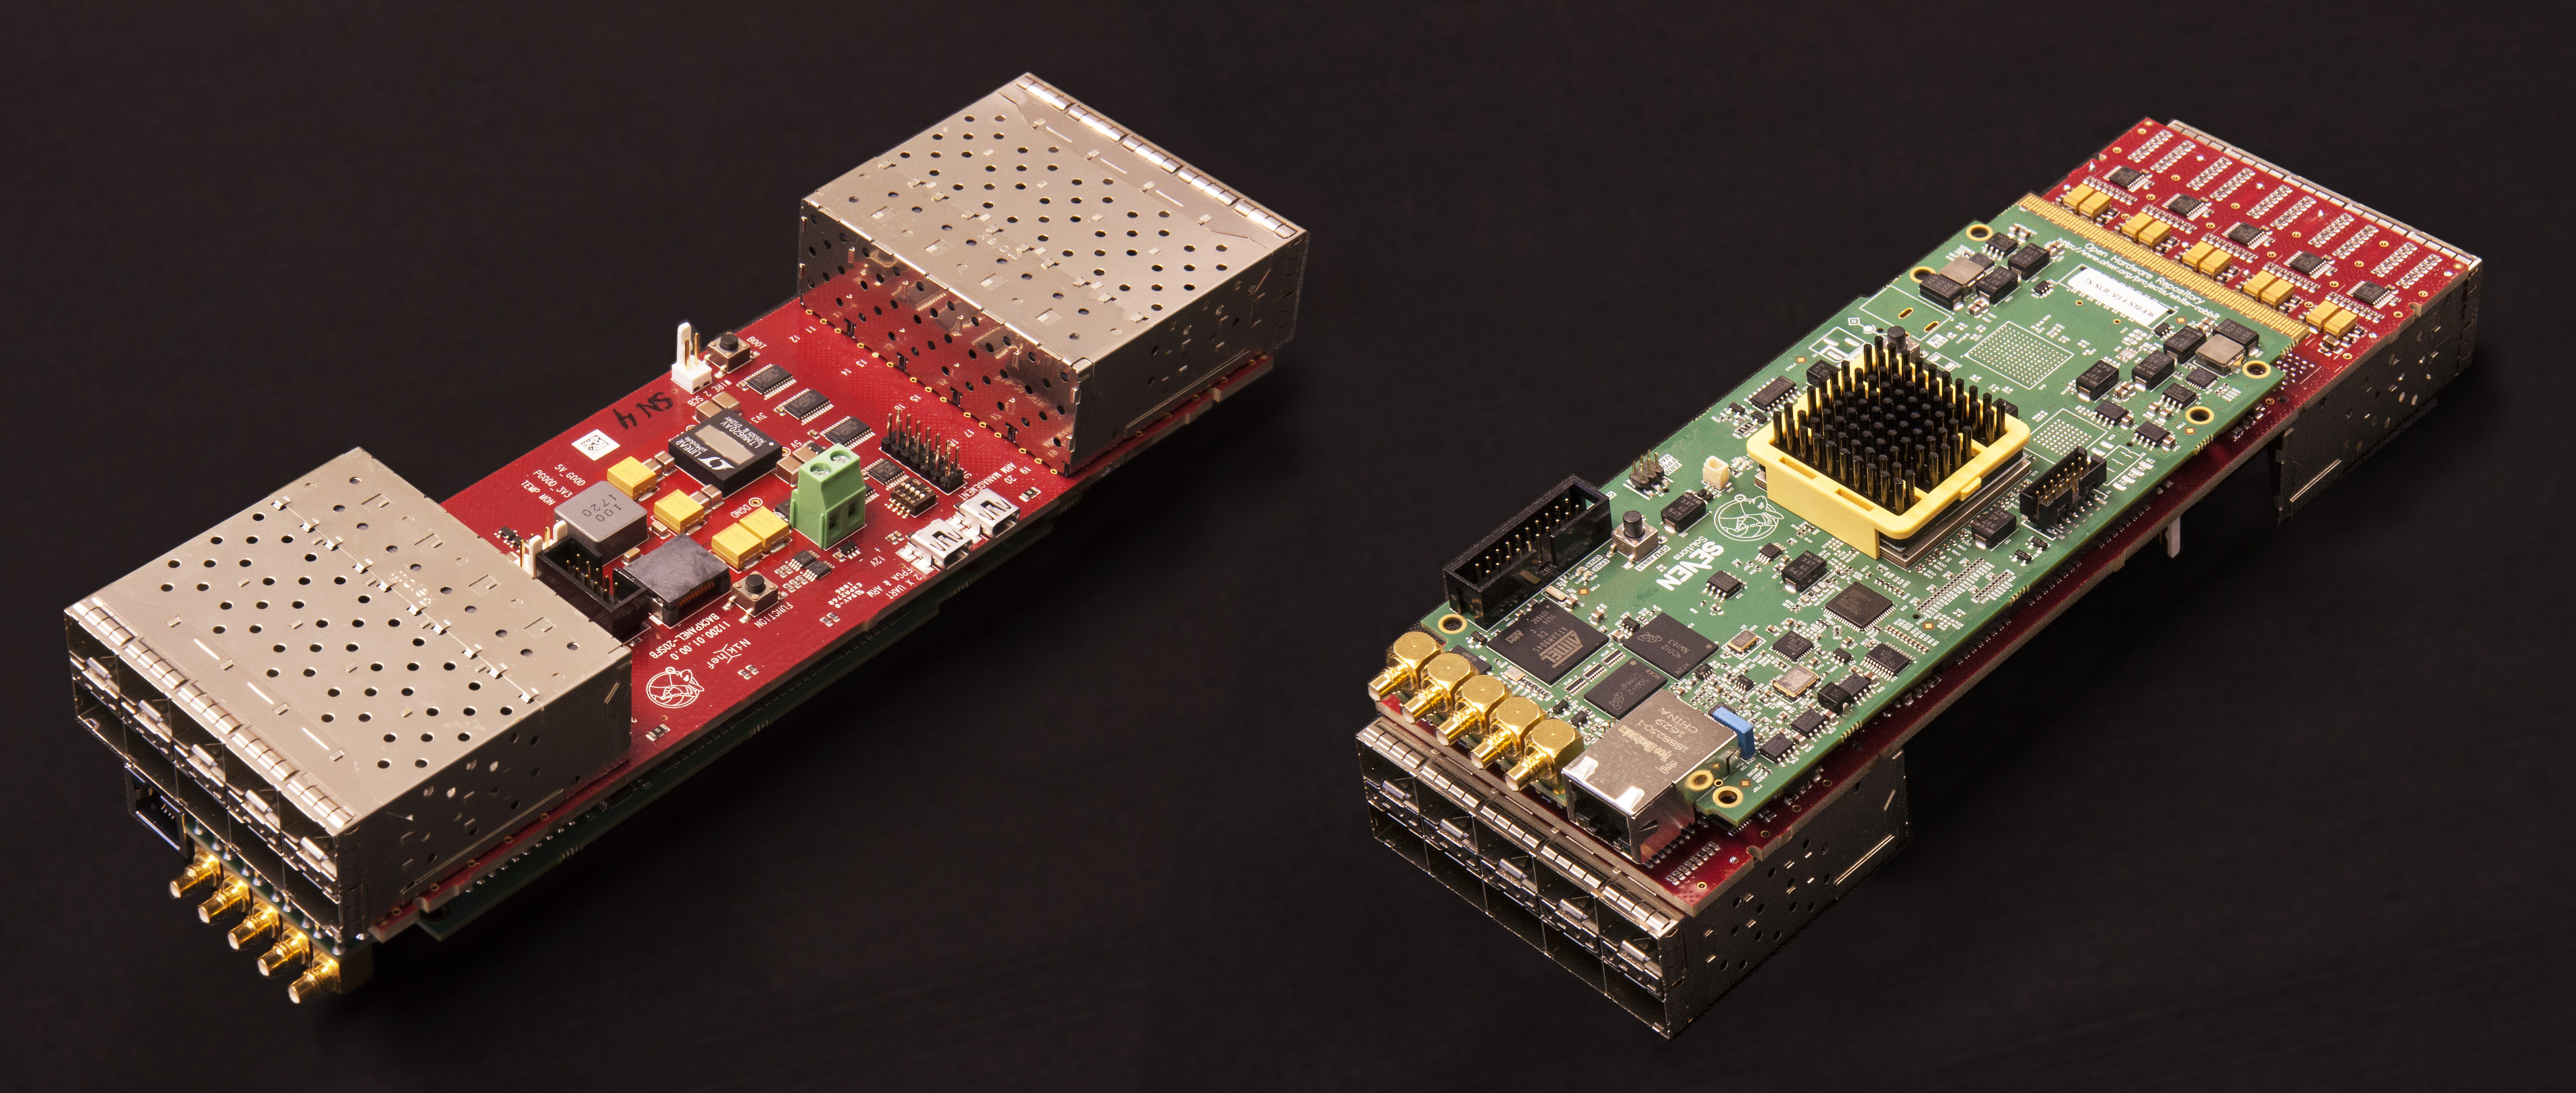
\includegraphics[height=6cm]{diagrams/5-daq/wr_switch.jpg}%
    }
    \quad
    \subcaptionbox{White Rabbit LEN\label{fig:clb}}{%
        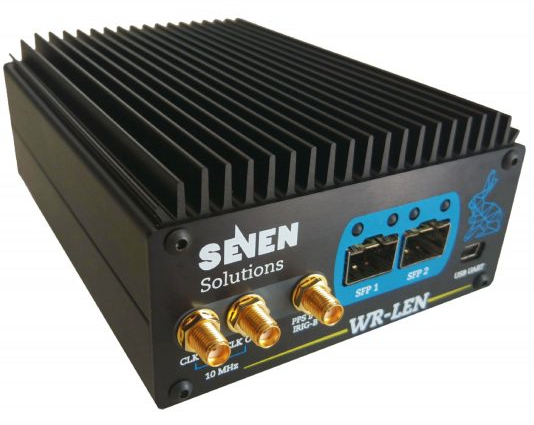
\includegraphics[height=6cm]{diagrams/5-daq/wr_len.jpg}%
    }
    \caption[Pictures of the White Rabbit timing hardware used within \chipsfive.]
    {Pictures of the White Rabbit timing hardware used within \chipsfive. A \emph{backplane-20SFP}
        version of a White rabbit switch, specially designed for \chips and KM3NeT is shown in
        (a), while the White Rabbit Lite Embedded Node (LEN) from Seven Solutions is shown in
        (b).}
\end{figure}

\begin{figure} % WHITE-RABBIT SYNC DIAGRAM %
    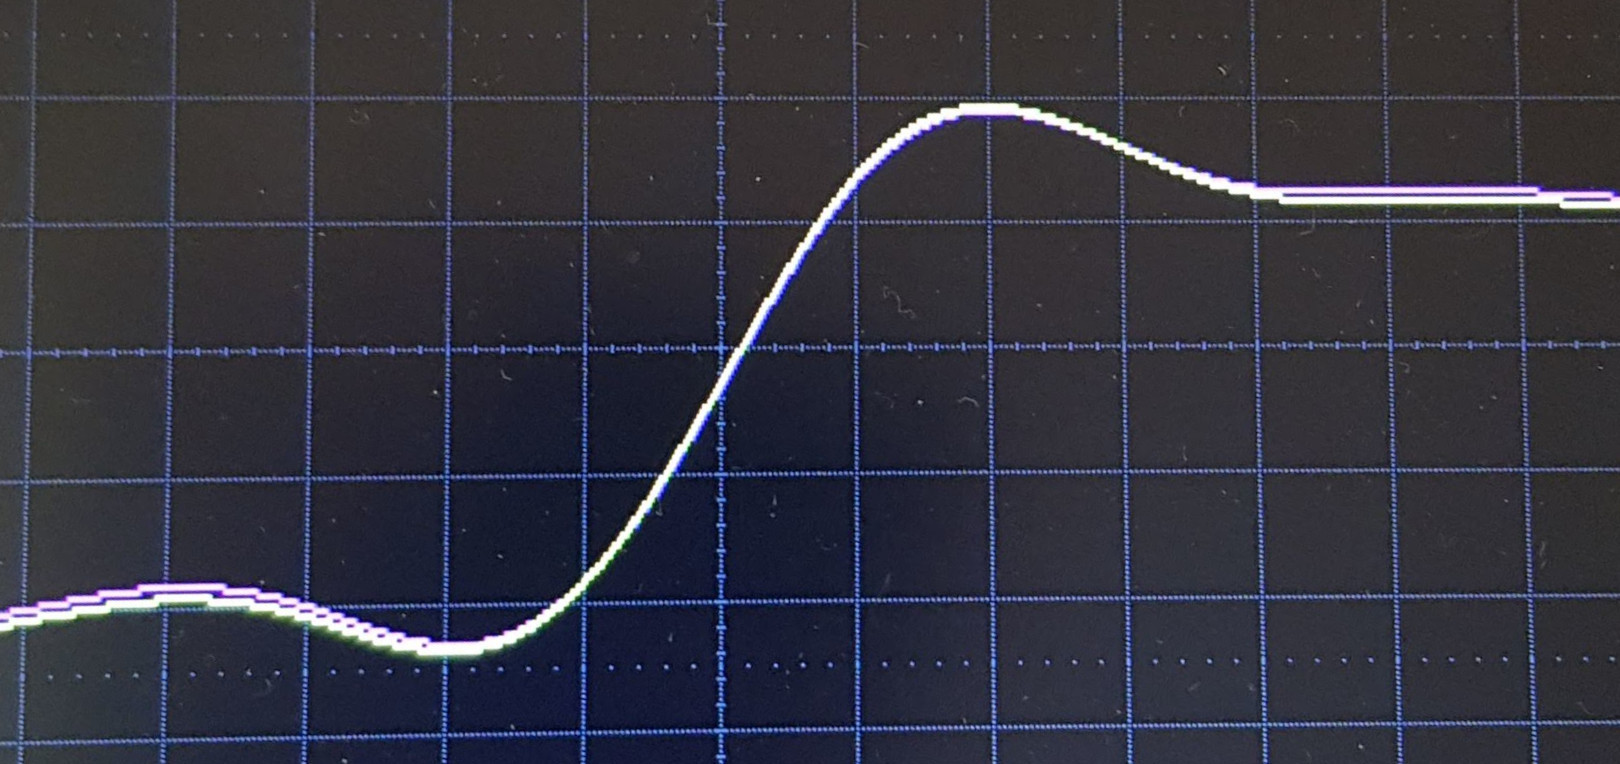
\includegraphics[width=0.8\textwidth]{diagrams/5-daq/sync.jpg}
    \caption[Picture of White Rabbit timing synchronisation seen in \chips.]
    {Picture of of oscilloscope measuring the \unit{10}{\mathrm{MHz}} White Rabbit signal of two
        switches shown in pink and yellow at either end of a \unit{500}{\mathrm{m}} long fibre.
        The vertical ticks are in nanoseconds showing the sub-nanosecond synchronisation possible
        with the White Rabbit timing system}
    \label{fig:sync}
\end{figure}

\section{Hardware} %%%%%%%%%%%%%%%%%%%%%%%%%%%%%%%%%%%%%%%%%%%%%%%%%%%%%%%%%%%%%%%%%%%%%%%%%%%%%%%
\label{sec:daq_hard} %%%%%%%%%%%%%%%%%%%%%%%%%%%%%%%%%%%%%%%%%%%%%%%%%%%%%%%%%%%%%%%%%%%%%%%%%%%%%

- Start from the bottom and work our way up!
- The task is to take TOT recorded hits, that are timestamped using the white-rabbit stuff and get
them to storage at Fermilab, all sorted, without losses, in a timely manner.
- Talk about general time resolution of the PMTs etc in the context of the overall time resolution
with the white rabbit.

\begin{figure} % TOT DIAGRAM DIAGRAM %
    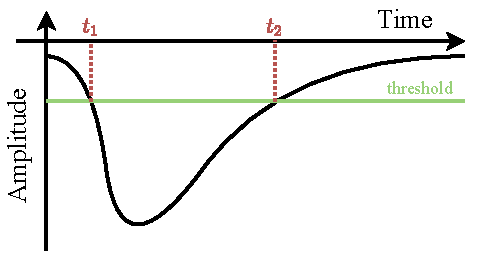
\includegraphics[width=0.7\textwidth]{diagrams/5-daq/tot.pdf}
    \caption[Illustrative diagram showing how time-over-threshold is measured.]
    {Illustrative diagram showing how time-over-threshold is measured. As soon as the rising edge
        of the charge pulse from a photon cascade passes a threshold a time is recorded, when the
        falling edge passes the threshold again a second time is recorded. The difference in time
        is output by the electronics as the time-over-threshold value.}
    \label{fig:tot}
\end{figure}

\begin{figure} % DAQ DIAGRAM %
    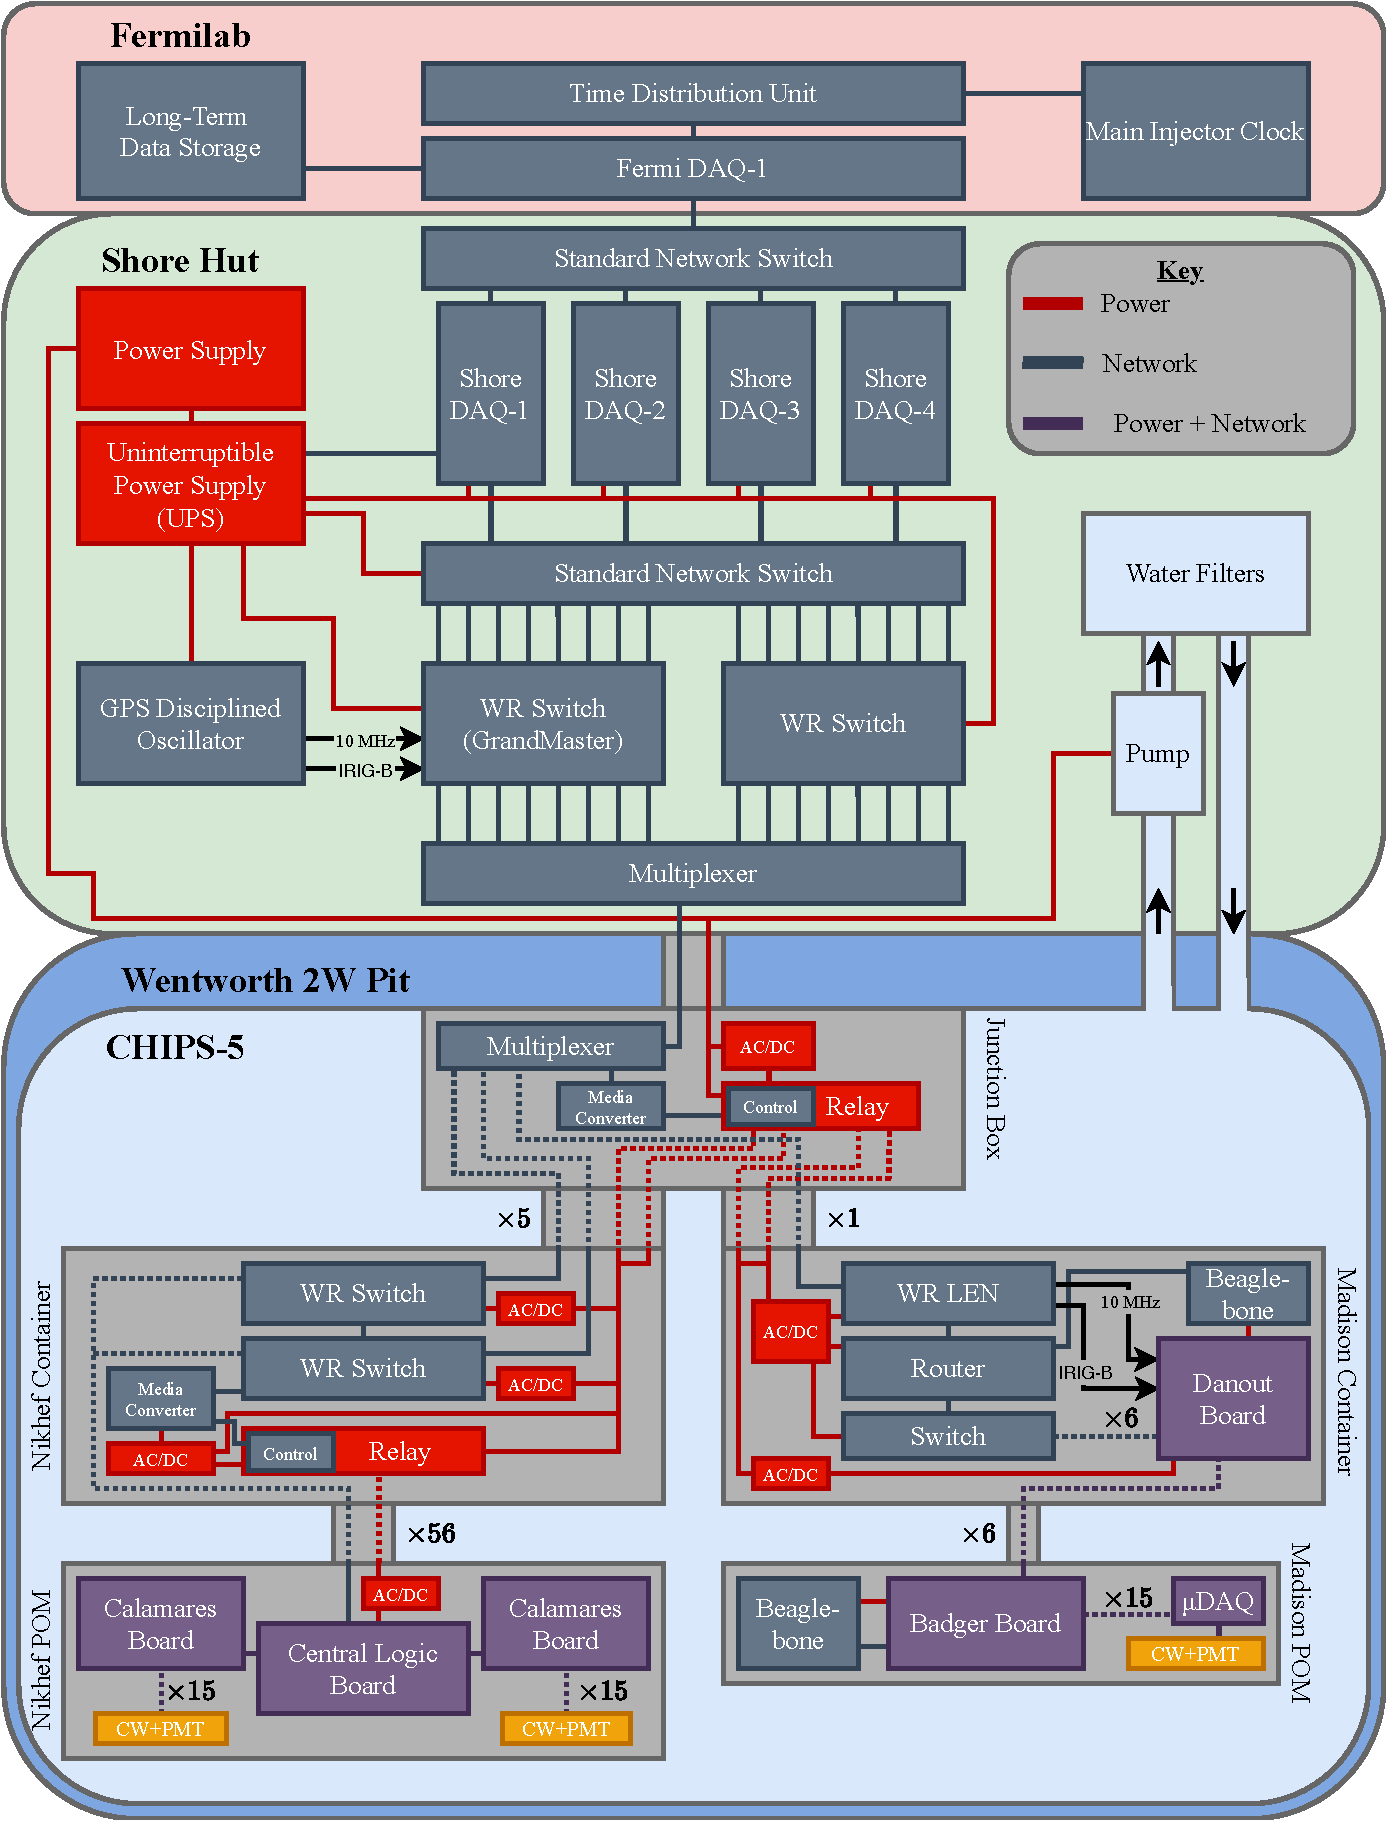
\includegraphics[width=\textwidth]{diagrams/5-daq/daq.pdf}
    \caption[Diagram of the \chipsfive data acquisition and power distribution system.]
    {Diagram of the \chipsfive DAQ and power distribution system.}
    \label{fig:daq}
\end{figure}

\begin{figure} % FULL SETUP DIAGRAM %
    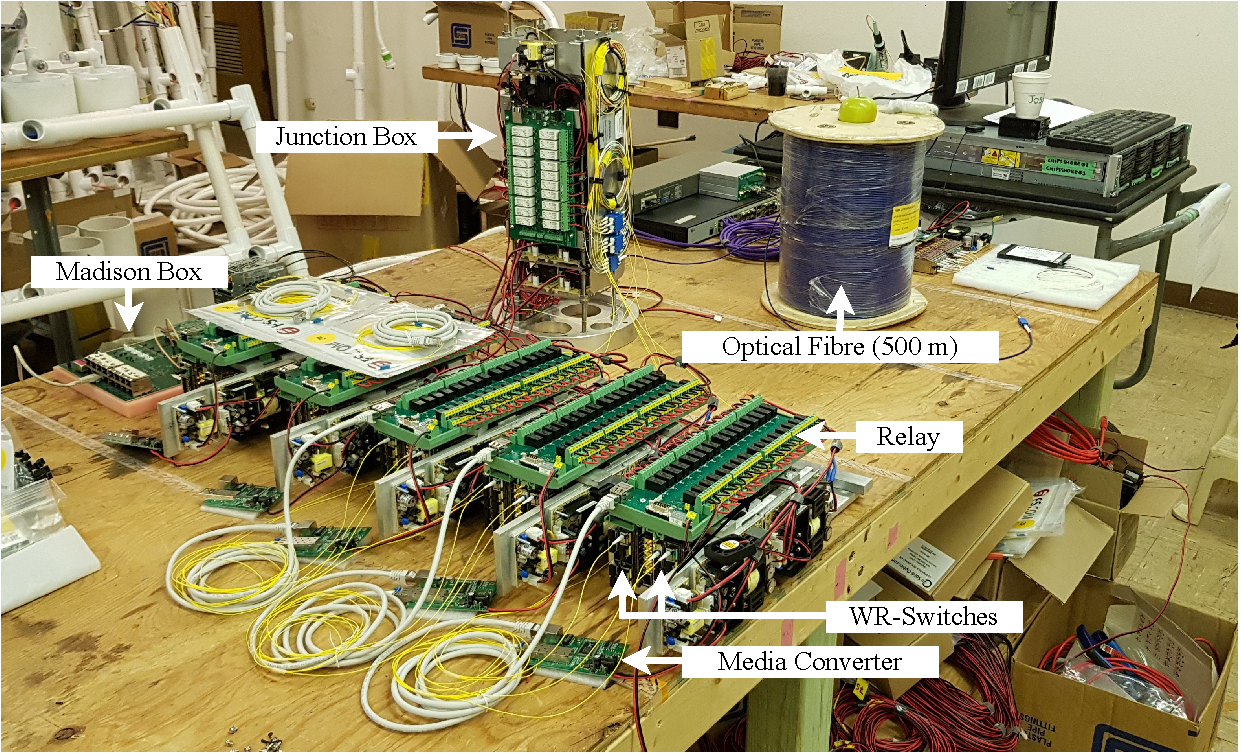
\includegraphics[width=\textwidth]{diagrams/5-daq/full_setup.pdf}
    %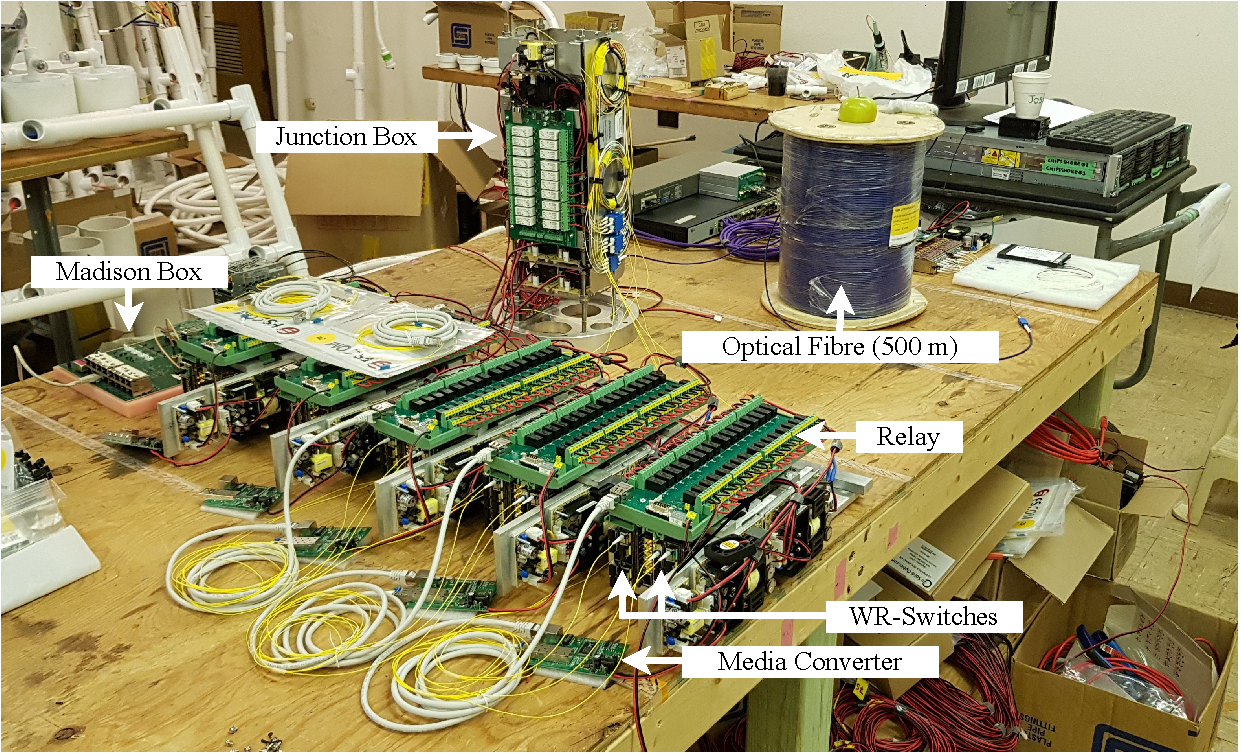
\includegraphics[angle=90,origin=c,width=0.8\textwidth]{diagrams/5-daq/full_setup.pdf}
    \caption[full set up short]
    {Picture of the full \chipsfive DAQ system}
    \label{fig:full_setup}
\end{figure}

\subsection{Km3NET hardware} %%%%%%%%%%%%%%%%%%%%%%%%%%%%%%%%%%%%%%%%%%%%%%%%%%%%%%%%%%%%%%%%%%%%%
\label{sec:daq_hard_km3net} %%%%%%%%%%%%%%%%%%%%%%%%%%%%%%%%%%%%%%%%%%%%%%%%%%%%%%%%%%%%%%%%%%%%%%

- km3net daq ref in~\cite{biagi2015, adrian2016, eijk2015}

\begin{figure} % NIKHEF PLANE DIAGRAM %
    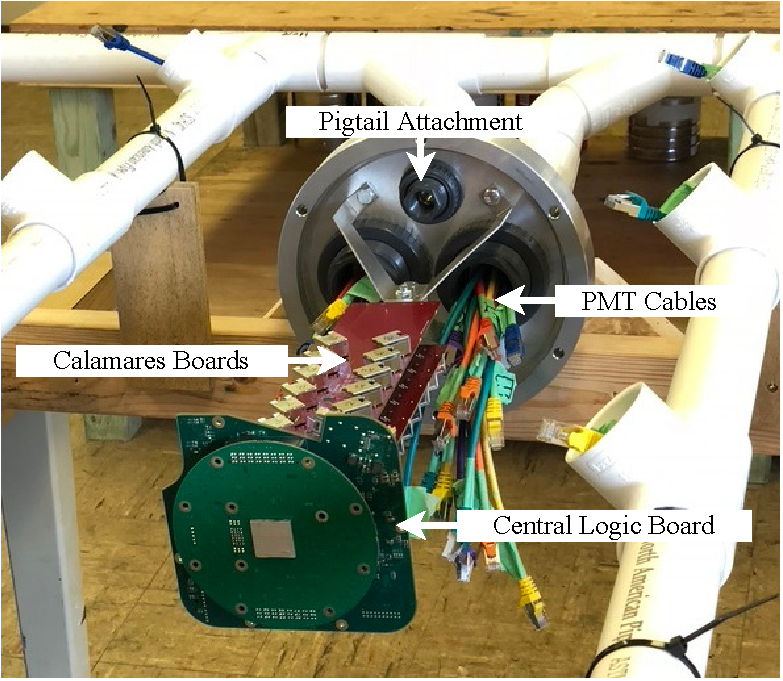
\includegraphics[width=0.8\textwidth]{diagrams/5-daq/nikhef_plane.pdf}
    \caption[nikhef plane short]
    {nikhef plane long}
    \label{fig:nikhef_plane}
\end{figure}

\subsection{Madison hardware} %%%%%%%%%%%%%%%%%%%%%%%%%%%%%%%%%%%%%%%%%%%%%%%%%%%%%%%%%%%%%%%%%%%%
\label{sec:daq_hard_madison} %%%%%%%%%%%%%%%%%%%%%%%%%%%%%%%%%%%%%%%%%%%%%%%%%%%%%%%%%%%%%%%%%%%%%

- Daan short ref in~\cite{eijk2018}
- Seven Solutions WR-LEN ref in~\cite{wrlen2020}
- Beaglebone ref in~\cite{beagle2020}

\begin{figure} % MADISON BOX DIAGRAM %
    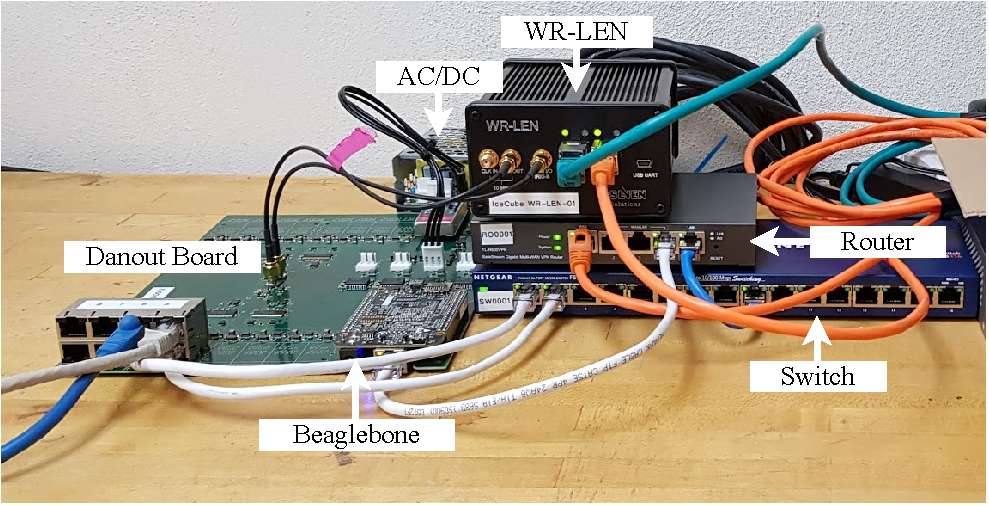
\includegraphics[width=\textwidth]{diagrams/5-daq/madison_box.pdf}
    \caption[madison box short]
    {madison box long}
    \label{fig:madison_box}
\end{figure}

\begin{figure} % MADISON PLANE DIAGRAM %
    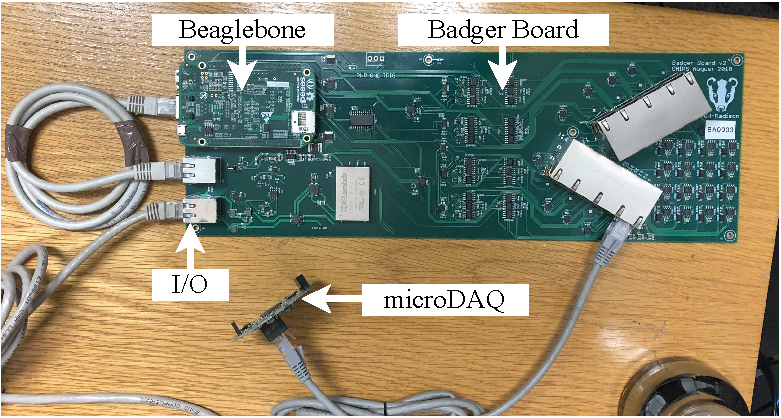
\includegraphics[width=0.8\textwidth]{diagrams/5-daq/madison_plane.pdf}
    \caption[madison plane short]
    {madison plane long}

    \label{fig:madison_plane}
\end{figure}

\subsection{Combined systems} %%%%%%%%%%%%%%%%%%%%%%%%%%%%%%%%%%%%%%%%%%%%%%%%%%%%%%%%%%%%%%%%%%%%
\label{sec:daq_hard_combined} %%%%%%%%%%%%%%%%%%%%%%%%%%%%%%%%%%%%%%%%%%%%%%%%%%%%%%%%%%%%%%%%%%%%

- White rabbit switch ref in~\cite{wrswitch2020}
- Multiplexer allows for 16 different channels using wavelengths between 1310nm and 1550nm with
corresponding SFPs (Small Form-Factor Pluggable Transceiver)

\begin{figure} % MANIFOLD DIAGRAM %
    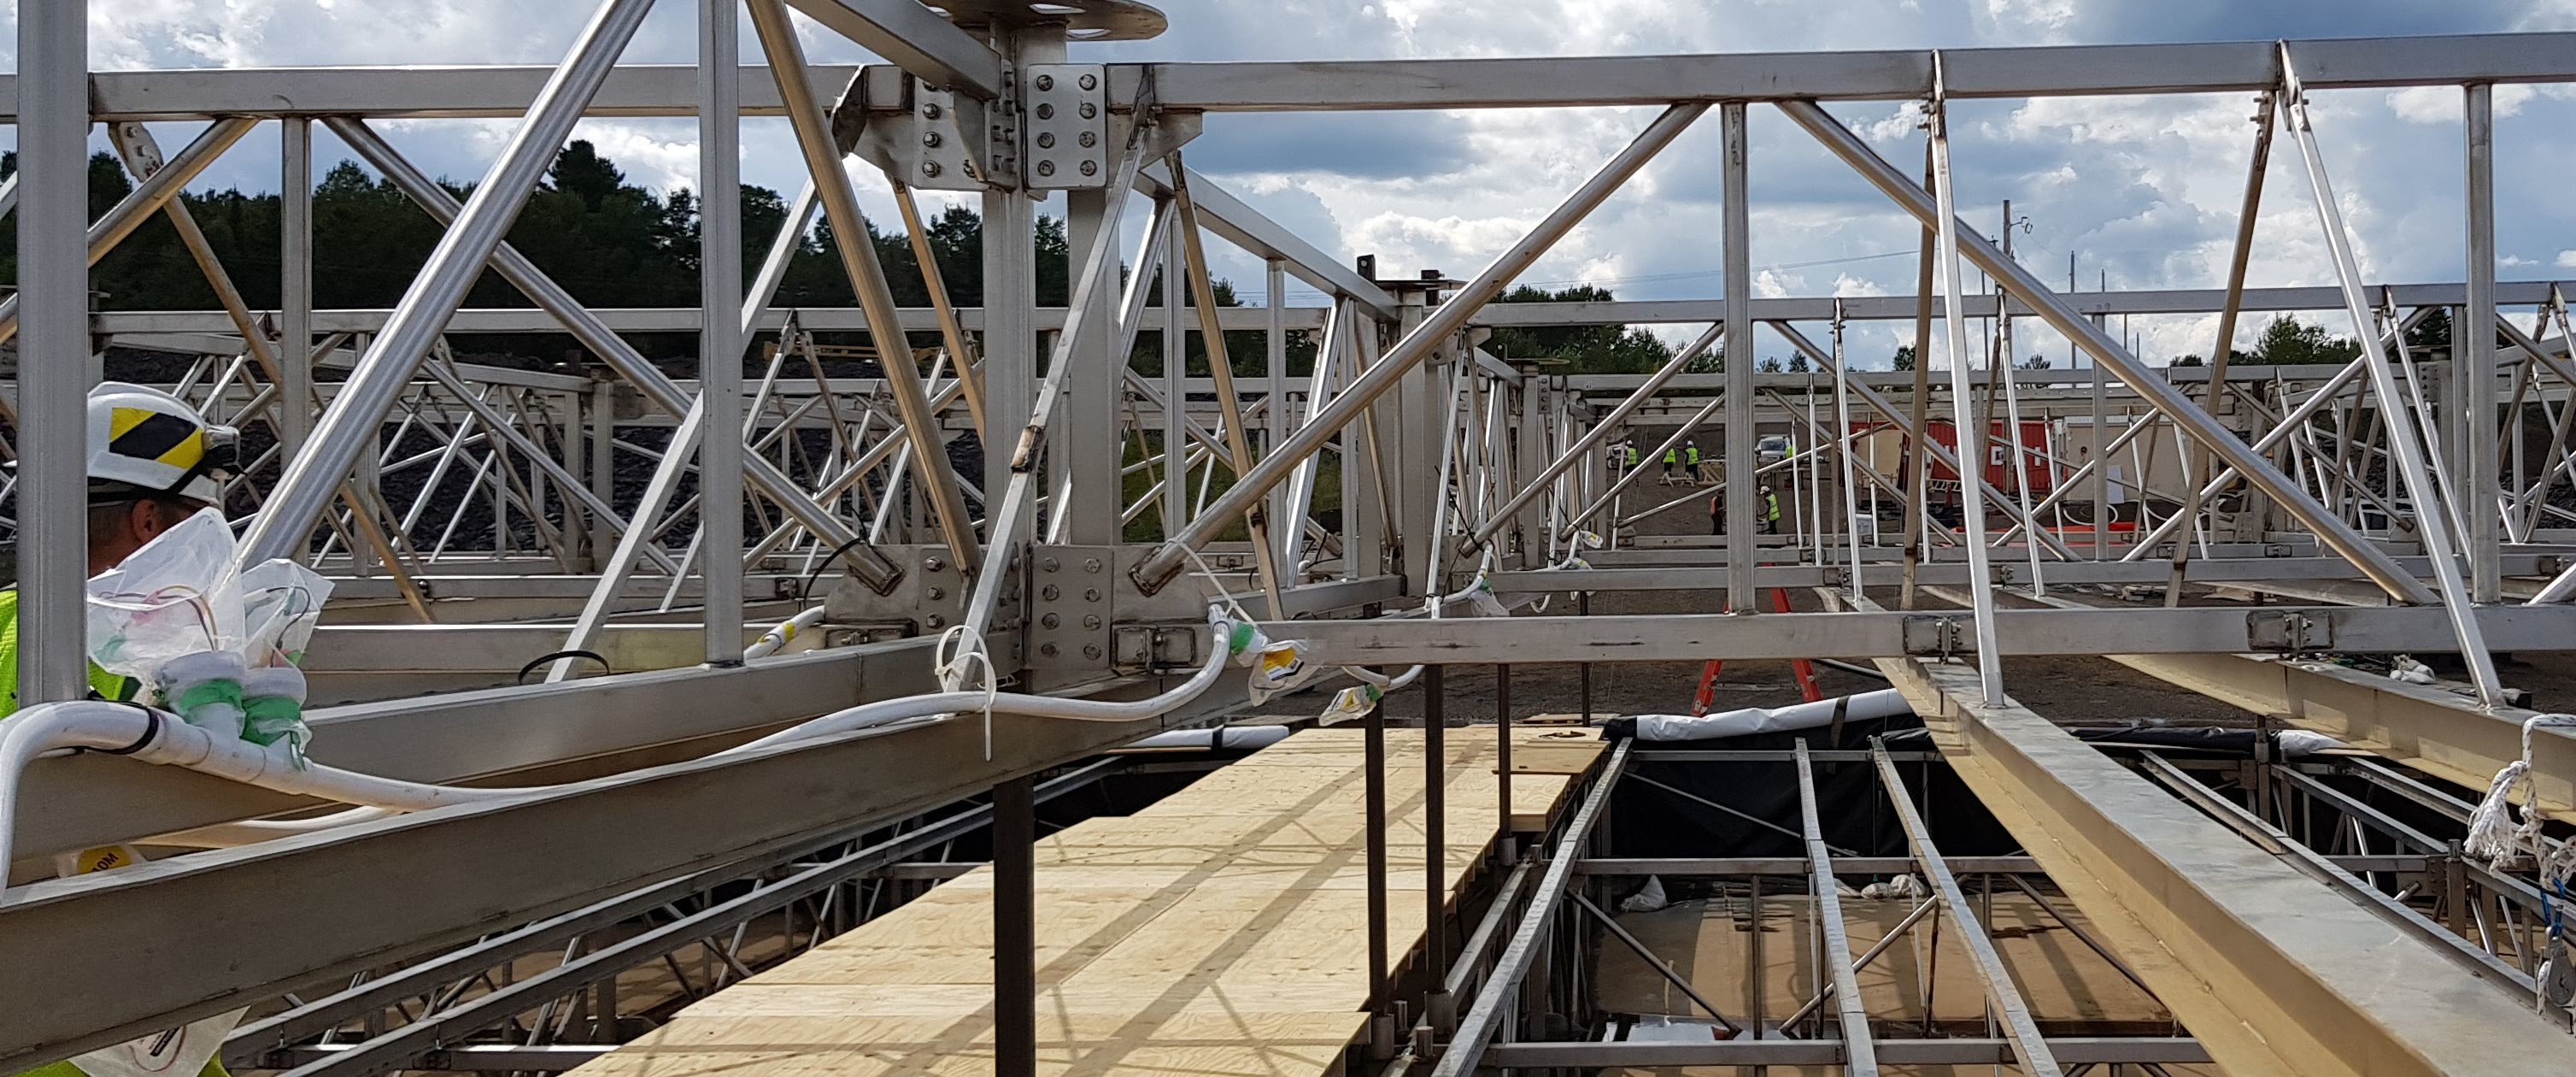
\includegraphics[width=\textwidth]{diagrams/5-daq/manifold.jpg}
    \caption[manifold short]
    {manifold long}
    \label{fig:manifold}
\end{figure}


\begin{figure} % JELLY DIAGRAM %
    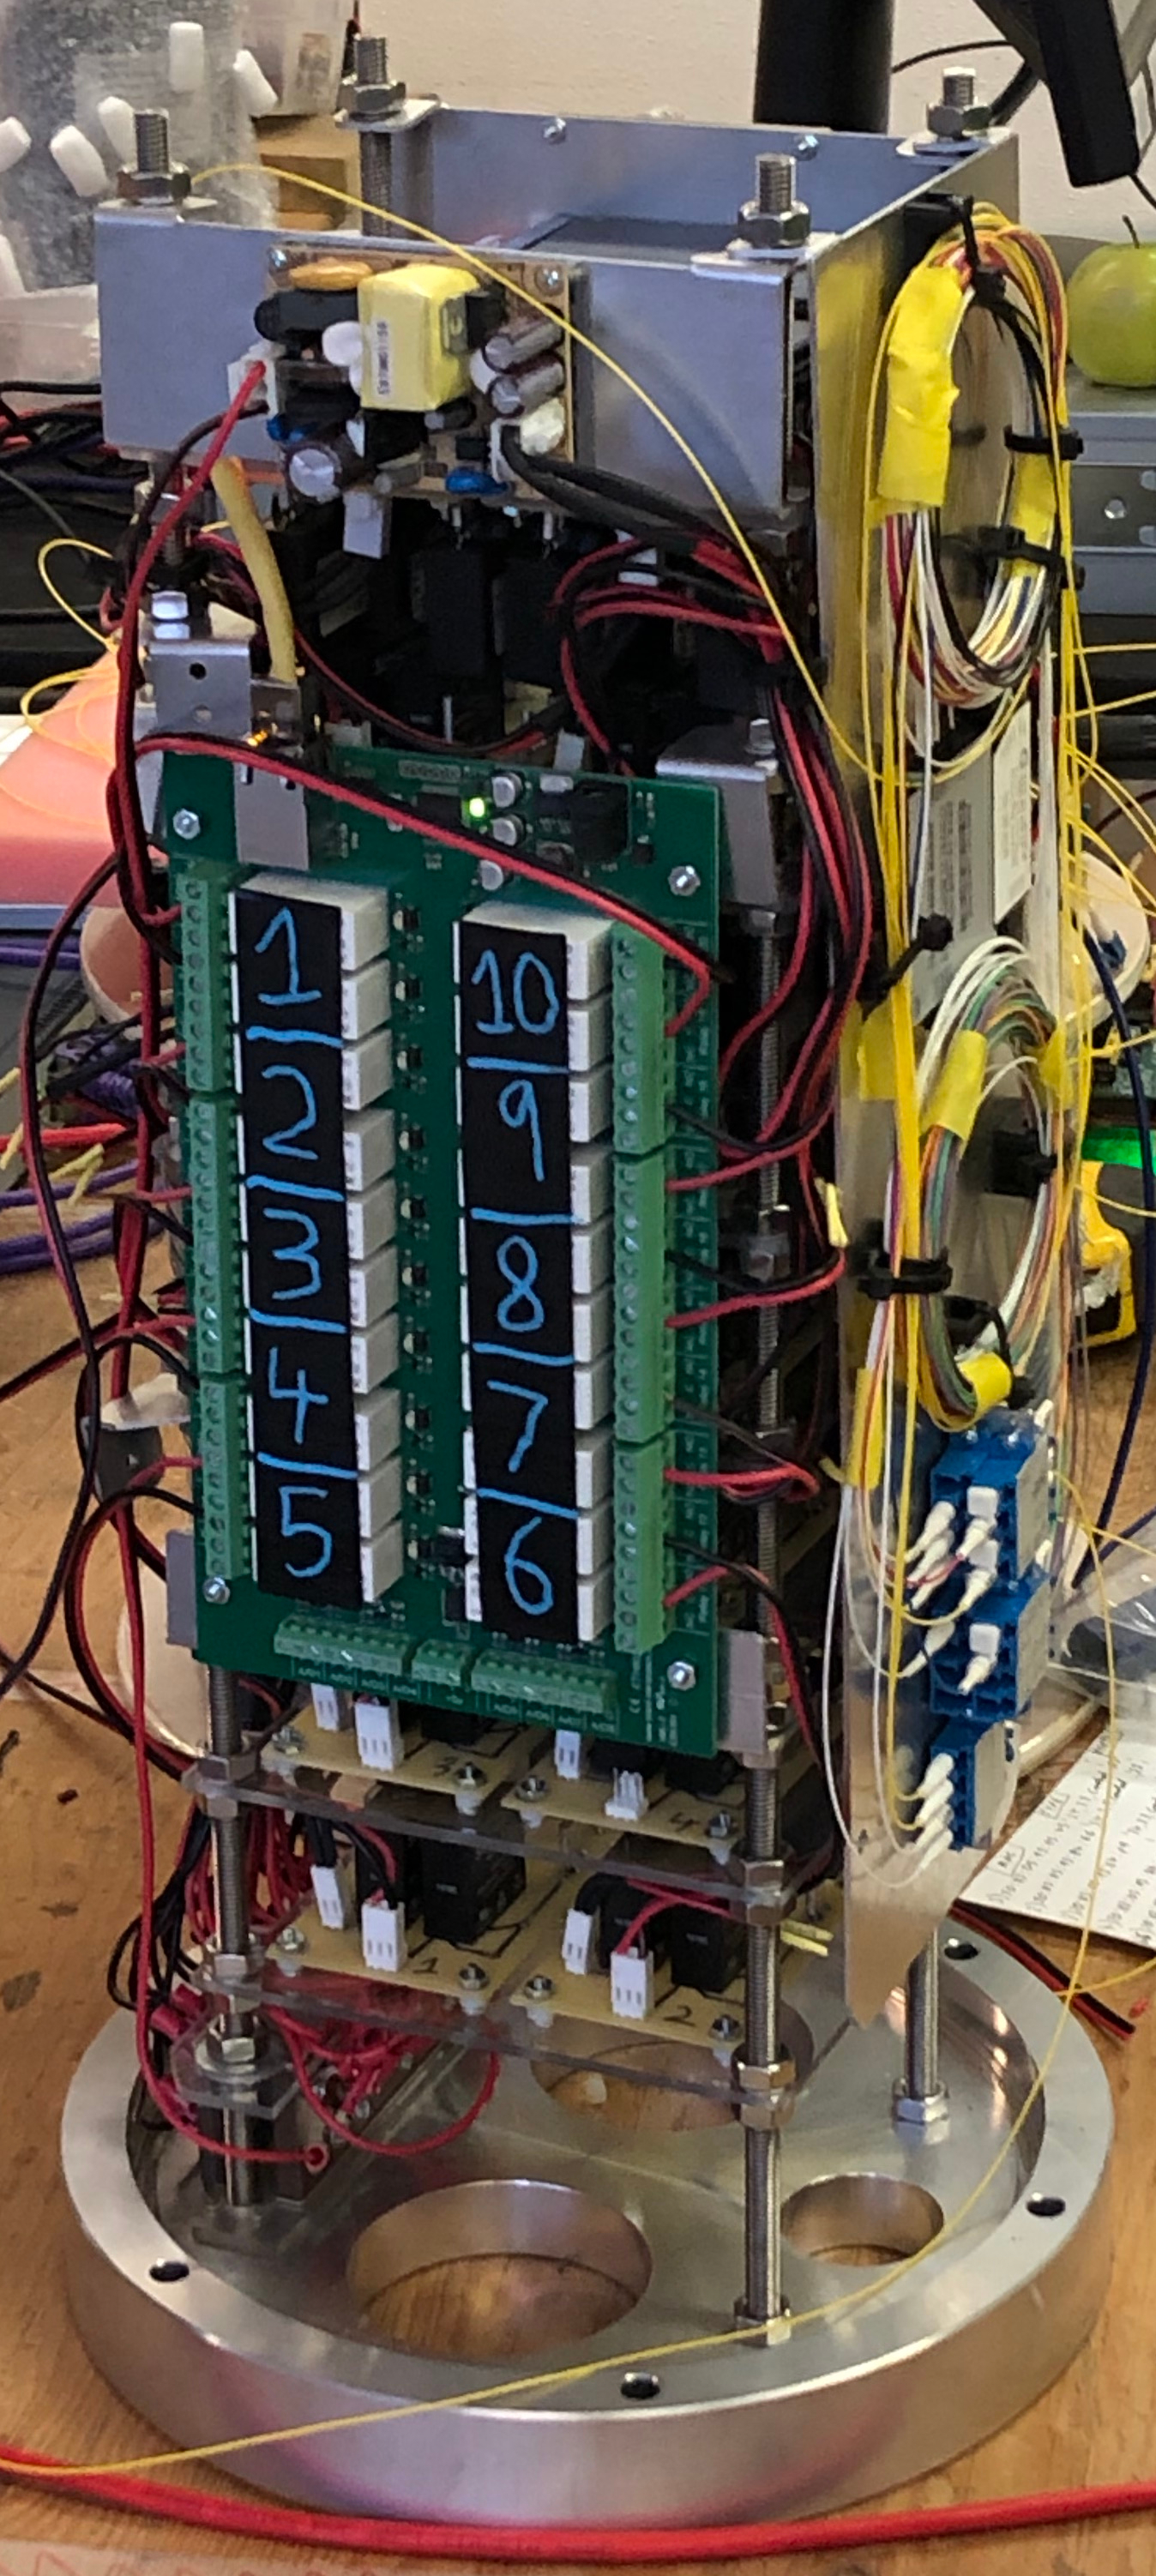
\includegraphics[width=0.5\textwidth]{diagrams/5-daq/jelly.jpeg}
    \caption[jelly short]
    {jelly long}
    \label{fig:jelly}
\end{figure}

\begin{figure} % WHITE-RABBIT GM SETUP DIAGRAM %
    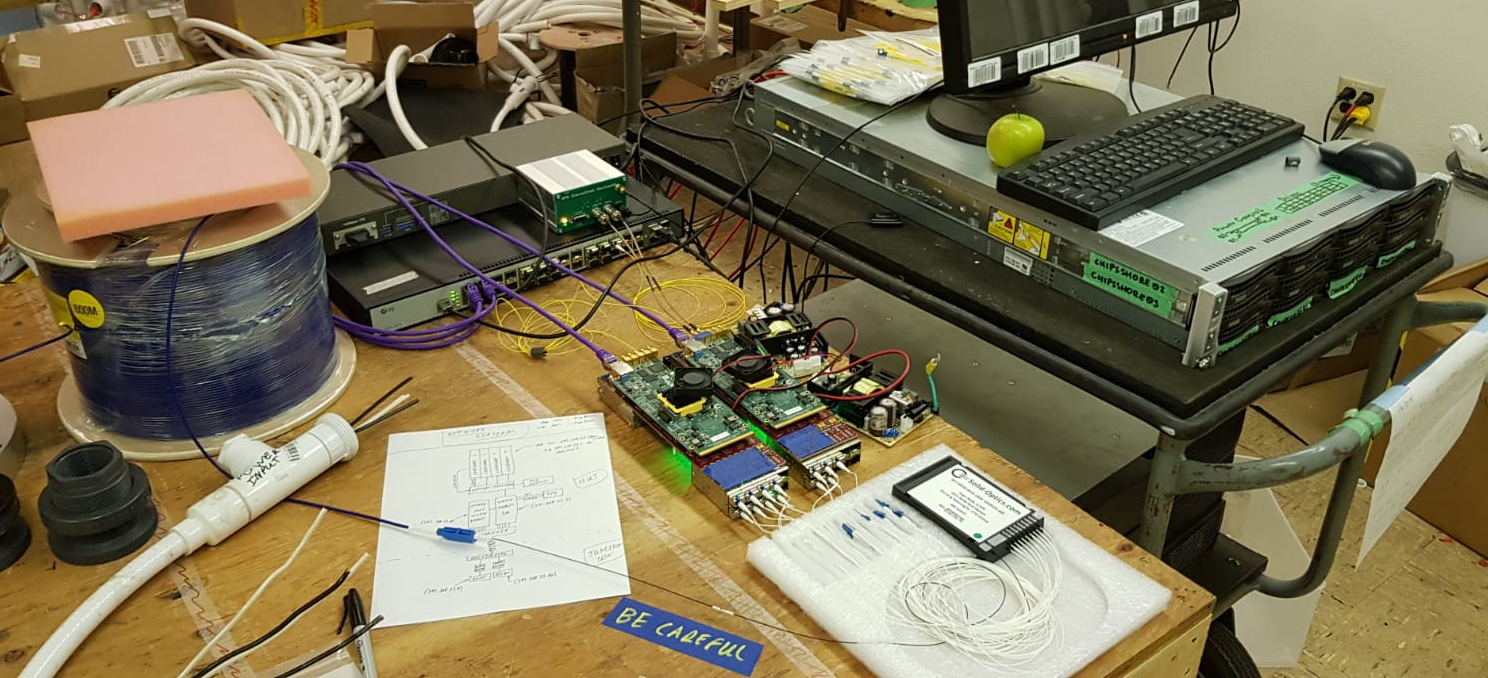
\includegraphics[width=\textwidth]{diagrams/5-daq/hut_daq.jpg}
    \caption[hut daq short]
    {hut daq long}
    \label{fig:hut_daq}
\end{figure}

\section{Data flow and software} %%%%%%%%%%%%%%%%%%%%%%%%%%%%%%%%%%%%%%%%%%%%%%%%%%%%%%%%%%%%%%%%%
\label{sec:daq_soft} %%%%%%%%%%%%%%%%%%%%%%%%%%%%%%%%%%%%%%%%%%%%%%%%%%%%%%%%%%%%%%%%%%%%%%%%%%%%%

DIAGRAM: Software diagram + finite state machine

- An `all-data-to-shore' approach as done in KM3NeT
- Data is sent in UDP packets (not TCP so some will go missing)
- microDAQ software repository with fh-library (field-hub) novel communication library
in~\cite{microdaq2020}. Most of Madison code is written in c!
- Mainly written in C++, full asynchronous using the BOOST Asio library in~\cite{boost2020} which
is a library for network and low-level I/O programming using an asynchronous model.
- Taking inspiration from the KM3NeT DAQ Java software
- The detector is configured using a single human readable configuration file that defines all the
POM types, MAC addresses, IP addresses, types, relay channels, which channels should be active and
their associate high voltage setting, threshold and electronic ID.
- Typical ethernet frame has a maximum transmission unit (MTU) size of 1500 bytes, we use Jumbo
frames that allow for an MTU of 9000 bytes, this means we have a lot less small frames with only a
limited number of recorded hits, which proved to be taxing to the switches and lead to an increase
in the number of dropped frames.
- 1Gb links between WR switches, 10Gb link between FS switch and main DAQ machine. Provides
sufficient bandwidth, DO A SMALL CALCULATION!

\subsection{The beam spill} %%%%%%%%%%%%%%%%%%%%%%%%%%%%%%%%%%%%%%%%%%%%%%%%%%%%%%%%%%%%%%%%%%%%%%
\label{sec:daq_soft_spill} %%%%%%%%%%%%%%%%%%%%%%%%%%%%%%%%%%%%%%%%%%%%%%%%%%%%%%%%%%%%%%%%%%%%%%%

\subsection{Hit acquisition and handling} %%%%%%%%%%%%%%%%%%%%%%%%%%%%%%%%%%%%%%%%%%%%%%%%%%%%%%%%
\label{sec:daq_soft_hits} %%%%%%%%%%%%%%%%%%%%%%%%%%%%%%%%%%%%%%%%%%%%%%%%%%%%%%%%%%%%%%%%%%%%%%%%

\subsection{Detector and data quality monitoring} %%%%%%%%%%%%%%%%%%%%%%%%%%%%%%%%%%%%%%%%%%%%%%%%
\label{sec:daq_soft_monitor} %%%%%%%%%%%%%%%%%%%%%%%%%%%%%%%%%%%%%%%%%%%%%%%%%%%%%%%%%%%%%%%%%%%%%

- Elasticsearch ref in~\cite{elastic2020}
- An open source RESTful, JSON-based, search engine and noSQL database.
- Data is stored in \emph{indices} in individual \emph{documents}
- Get to leverage an enormous amount of online support and the community
- daqlog: Uses for DAQ application logging with a severity
- daqstate: Used to report the current state of various DAQ applications
- monpom: Used for reporting general POM monitoring information, such as temp, humidity, status
- monchannel: Used for reporting individual channel monitoring, such as rate, veto
- A series of altering rules are also setup constantly monitoring the status of the monitoring
data contained within the elasticsearch database to alert via slack or email individuals if something goes wrong.
- We index asynchronously to not block data taking, all data is backed up easily.
- Use the Kibana user interface which is accessible through a browser, means that no special
equipment, or GUIs are used, anyone on any machine has access to the full monitoring stack from
their browser. A series of dashboards ar setup to monitor everything within the detector.
- A series of indices are setup to store data which is sent via standard REST messages to the
database, the special indexing allows for quick `searching' over any time period etc... for
monitoring.
- Also means that anyone can quikcly/easily look at any part of the data and make plots etc...
without needing to write an additional part of a monitoring program.


\begin{figure} % MONITORING DIAGRAM %
    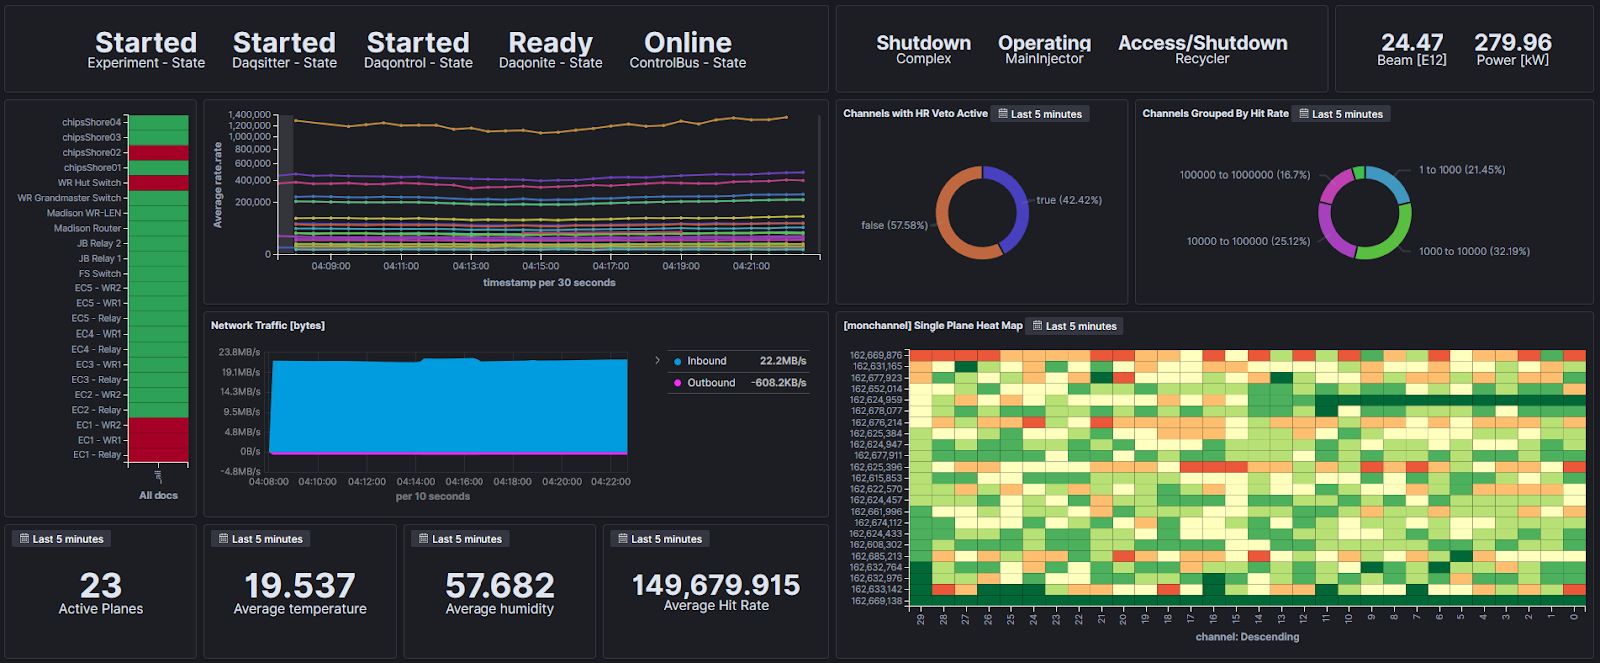
\includegraphics[width=\textwidth]{diagrams/5-daq/monitoring.png}
    \caption[monitoring short]
    {monitoring long}
    \label{fig:monitoring}
\end{figure}